\documentclass{standalone}
% translate with >> pdflatex -shell-escape <file>

% This file is an extract of the PGFPLOTS manual, copyright by Christian Feuersaenger.
% 
% Feel free to use it as long as you cite the pgfplots manual properly.
%
% See
%   http://pgfplots.sourceforge.net/pgfplots.pdf
% for the complete manual.
%
% Any required input files (for <plot table> or <plot file> or the table package) can be downloaded
% at
% http://www.ctan.org/tex-archive/graphics/pgf/contrib/pgfplots/doc/latex/
% and
% http://www.ctan.org/tex-archive/graphics/pgf/contrib/pgfplots/doc/latex/plotdata/

\usepackage{pgfplots}
\usepackage{pgfplotstable}
\pgfplotsset{compat=newest}

% The manual loads these libraries globally; the extracted standalone examples
% need them too. external/clickable/snakes are intentionally omitted.
\usetikzlibrary{
	arrows.meta,backgrounds,calc,decorations.footprints,decorations.markings,
	decorations.pathreplacing,fixedpointarithmetic,intersections,patterns,
	plotmarks,shapes.arrows,spy,through}
\usepgfplotslibrary{
	colorbrewer,colormaps,dateplot,fillbetween,groupplots,patchplots,polar,
	smithchart,statistics,ternary,units}

% Some colormap examples reuse this display style defined earlier in the manual.
\pgfplotsset{
	cycle from colormap manual style/.style={
		x=3cm,y=10pt,ytick=\empty,
		colorbar style={x=,y=,ytick=\empty},
		point meta min=0,point meta max=1,
		stack plots=y,
		y dir=reverse,colorbar style={y dir=reverse},
		every axis plot/.style={line width=2pt},
		legend entries={0,...,20},
		legend pos=outer north east,
	},
}

\pagestyle{empty}

\begin{document}
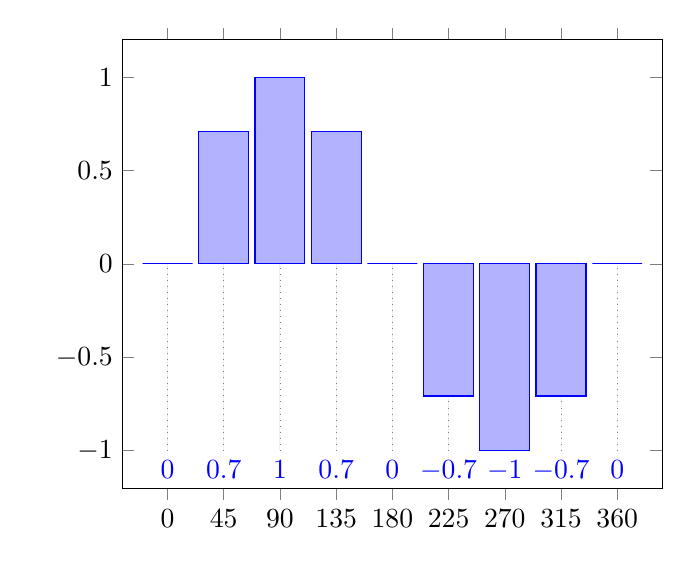
\begin{tikzpicture}
\begin{axis}[
    ybar,
    nodes near coords,
    %
    % we want to provide absolute 'at' values
    % for the nodes:
    scatter/position=absolute,
    every node near coord/.style={
        at={(\pgfkeysvalueof{/data point/x},-1)},
        % pretty printing:
        anchor=north,
        /pgf/number format/fixed,
        /pgf/number format/precision=1,
        % assign a name which can be referenced below:
        name=NNC\pgfkeysvalueof{/data point/index},
    },
    % ... draw a dotted line between
    % the marker and the bar:
    /pgfplots/scatter/@post marker code/.add code={}{
        \draw [dotted,help lines]
            (NNC\pgfkeysvalueof{/data point/index})
            -- (\pgfkeysvalueof{/data point/x},
            {min(0,\pgfkeysvalueof{/data point/y})});
    },
    % assign suitable tick labels:
    xtick=data,
]
    % some dummy data:
    \addplot+ [
        domain=0:360,
        bar width=360/9,
        samples=9,
    ] {sin(x)};
\end{axis}
\end{tikzpicture}
\end{document}
